\section{MODELING}

In this section, we describe the dynamic model and control of a basic flapping-wing drone.

\subsection{Dynamic Model}

\begin{figure}[t]
    \centering
    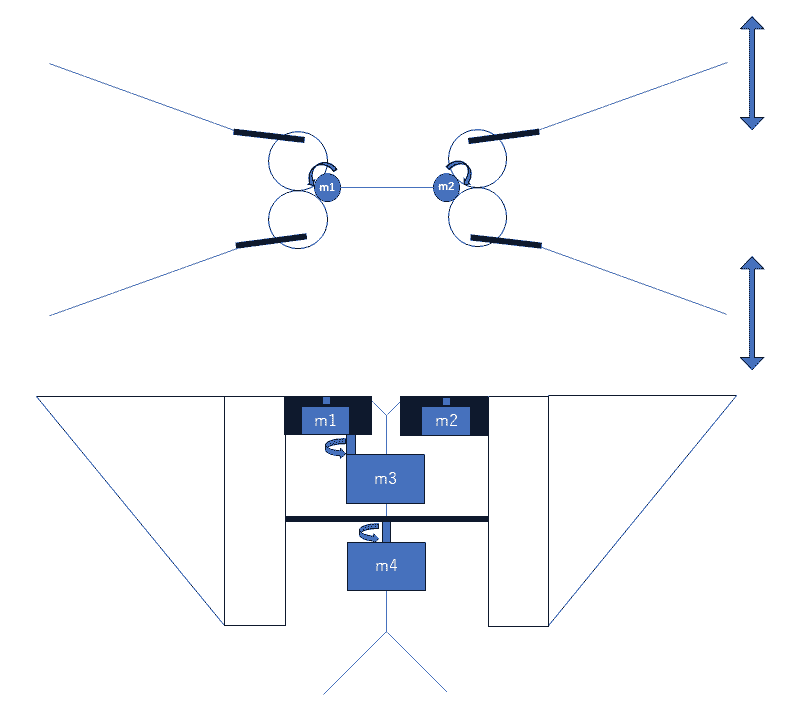
\includegraphics[width=\columnwidth]{modeling.png}
    \caption{The mechanical structure model of a flapping-wing drone. It has motors for thrust (m1, m2), a motor for wing orientation (m3), and a motor for yaw control (m4).}
    \label{figure:modeling}
  \end{figure}
  

Based on the model depicted in Fig. \ref{figure:modeling}, the threedimensional force $f_i$ generated by $m_i$ can be
written as:

\begin{equation}
    {}^{\{CoG\}}\bm{f_i} = {\lambda_i}^{\{CoG\}}\bm{u_i},
    \end{equation}
    
    \begin{equation}
    {}^{\{CoG\}}\bm{u_i} = {}^{\{CoG\}}R_{\{F_i\}}(\phi_i, \theta_i)
    \begin{bmatrix}
    0 \\
    0 \\
    1
    \end{bmatrix},
    \end{equation}
    
    where ${}^{\{CoG\}}R_{\{F_i\}}(q, \phi_i, \theta_i)$ is the rotation matrix of the motor frame
   {\{$F_i$\}} w.r.t. the frame ${\{CoG\}}$, and $\lambda_i$ is the thrust coefficient of the $m_i$. 
   $\phi_i$ and $\theta_i$ are rotational angles of the $m_3$ and $m_4$, respectively.
   The total force and torque generated by $m_1$ and $m_2$ can be written as:
    
    \begin{equation}
    \begin{bmatrix}
    {}^{\{CoG\}}\bm{f}_\lambda \\
    {}^{\{CoG\}}\bm{\tau}_\lambda
    \end{bmatrix}
    =
    \begin{bmatrix}
    \sum_{i=1}^{2} {}^{\{CoG\}}\bm{f}_i \\
    \sum_{i=1}^{2} {}^{\{CoG\}}\bm{p}_i \times {}^{\{CoG\}}\bm{f}_i
    \end{bmatrix}
    = Q\bm{\lambda},
    \end{equation}
    
    \begin{align}
    Q =
    \begin{bmatrix}
    {}^{\{CoG\}}\bm{u_1} & {}^{\{CoG\}}\bm{u_{2}} \\
    {}^{\{CoG\}}\bm{p_1} \times {}^{\{CoG\}}\bm{u_1} & {}^{\{CoG\}}\bm{p_{2}} \times {}^{\{CoG\}}\bm{u_{2}}
    \end{bmatrix}\notag\\
    \bm{\lambda} =
    \begin{bmatrix}
    \lambda_1 
    \quad
    \lambda_2
    \end{bmatrix}^T.
    \end{align}

    The whole dynamic model can be written as follows:

    \begin{equation}
      \label{linear}
        m^{\{W\}}\bm{\ddot{r}}_{\{CoG\}} = ^{\{W\}}R_{\{CoG\}} \bm{f}_{\lambda} - m \bm{g} + \sum_{i=1}^{N_c} {^{\{W\}} \bm{f}_{c_i}}, 
    \end{equation}
    
    \begin{equation}
      \label{angular}
        I \bm{\dot{\omega}} + \bm{\omega} \times I\bm{\omega}  = \bm{\tau}_{\lambda} + \sum_{i=1}^{N_c} {^{\{CoG\}} \bm{p}_{c_i} \times {^{\{W\}} R_{\{CoG\}}}^{T} {^{\{W\}} \bm{f}_{c_i}}},
    \end{equation}
    
    where $m$ is the mass of the drone, $I$ is the inertia matrix, $\bm{r}_{\{CoG\}}$ is the position of the center of gravity, $\bm{g}$ is the gravity vector, $\bm{f}_{c_i}$ is the contact force, and $\bm{p}_{c_i}$ is the position of the contact point.

\subsection{Control}

\begin{figure}[t]
  \centering
  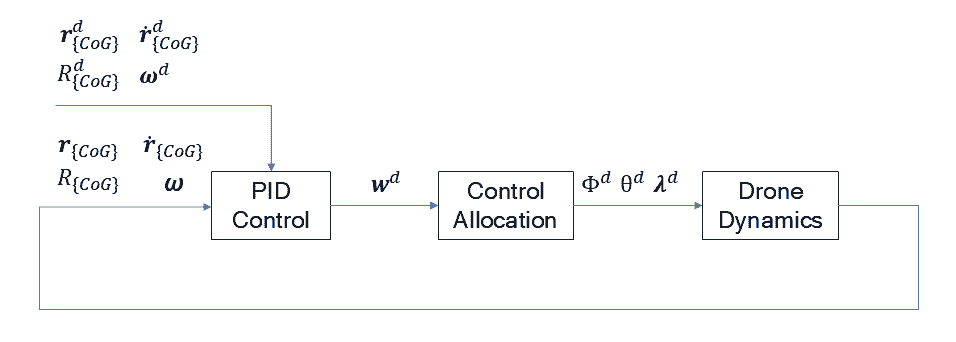
\includegraphics[width=\columnwidth]{control.png}
  \caption{The PID control model of a flapping-wing drone. It has mot}
  \label{figure:control}
\end{figure}

The control model of the flapping-wing drone is shown in Fig. \ref{figure:control}.
Based on the dynamics of (\ref{linear}) and (\ref{angular}), 
we can design a PID controller for the flapping-wing drone. 
One of the control inputs is the desired force $\bm{f}_{\lambda}^{d}$, which can be written as:

\begin{align}
  {}^{\{CoG\}} \bm{f}_{\lambda}^{d} = 
  & \quad m {^{\{W\}}R_{\{CoG\}}^{T}} 
  \left( K_{f,p} \bm{e_r} + K_{f,i} \int \bm{e_r} \, dt + K_{f,d} \bm{\dot{e}_r} \right) \notag \\
  & + {^{\{W\}}R_{\{CoG\}}^{T}} 
  \left( m\bm{g} - \sum_{i=1}^{N_c} {^{\{W\}} f_{c_i}} \right).
  \end{align}

where $K_{f,*}$, are the PID gain diagonal matrices, and $\bm{e_r} = {}^{\{W\}}\bm{r}_{\{CoG\}}^{d} - {}^{\{W\}}\bm{r}_{\{CoG\}}$ is the position error.

The attitude control follows the part of the control method
proposed by \cite{lee2010geometric}:

\begin{align}
  ^{\{CoG\}} \bm{\tau}_{\lambda}^{d} &= I 
  \left( K_{\tau,p} \bm{e}_R + K_{\tau,i} \int \bm{e}_R \, dt + K_{\tau,d} \bm{e}_{\bm{\omega}} \right) \notag \\
  & \quad + \bm{\omega} \times I \bm{\omega} - \sum_{i=1}^{N_c} \bm{p}_{c_i} \times R^T \bm{f}_{c_i},
  \end{align}
  
  \begin{equation}
  \bm{e}_R = \frac{1}{2} \left( R^T R^d - (R^d)^T R \right)^{\vee},
  \end{equation}
  
  \begin{equation}
  \bm{e}_{\omega} = R^T R^d \bm{\omega}^d - \bm{\omega}.
  \end{equation}

  Then, the desired wrench w.r.t the frame $\{CoG\}$ can be summarized as follows:

\begin{equation}
\bm{w}^d = \begin{bmatrix} ^{\{CoG\}} \bm{f}_{\lambda}^{d} \quad ^{\{CoG\}} \bm{\tau}_{\lambda}^{d} \end{bmatrix}^T. 
\end{equation}
  